\section{Results}
\label{sec:RESULTS_RESULTS}
\pcstart{s45}{2}

\subsection{Observed Distributions}
\label{sec:RESULTS_RESULTS_OBSERVED_DISTRIBUTIONS}

\Cref{fig:main-result} shows the [key observable] distribution.

\begin{figure}[htbp]
  \centering
  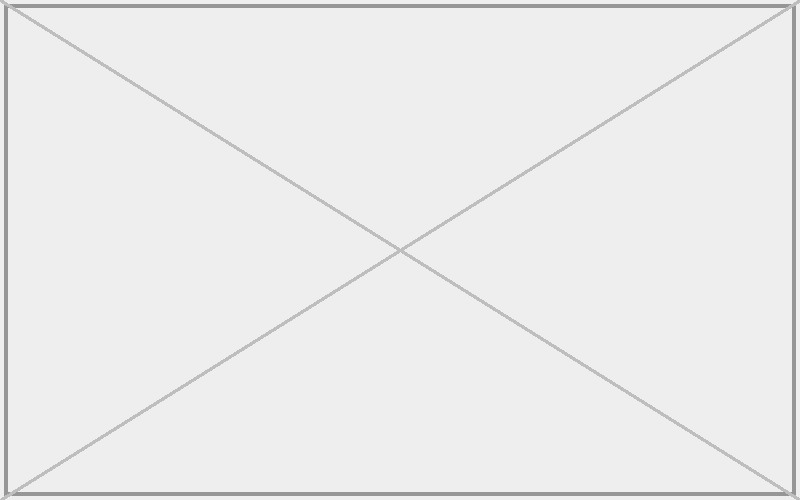
\includegraphics[width=0.7\textwidth]{figures/placeholder.png}
  \caption{Distribution of [observable] in data compared with the \gls{mc} prediction. [State the key takeaway.] \adaptedfrom{higgs-discovery}}
  \label{fig:main-result}
\end{figure}

\subsection{Signal Extraction}
\label{sec:RESULTS_RESULTS_SIGNAL_EXTRACTION}

The signal yield is extracted using [method]:
\begin{equation}
  N_{signal} = [value] \pm [stat] \pm [syst]
  \label{eq:signal-yield}
\end{equation}

\subsection{Measurement}
\label{sec:RESULTS_RESULTS_MEASUREMENT}

The measured [cross section/branching ratio/etc.] is:
\begin{equation}
  \sigma \times BR = [value] \pm [stat] \pm [syst] \text{ pb}
  \label{eq:measurement}
\end{equation}

This result is consistent with the Standard Model prediction of [value] pb.

\pcend{s45}
